\section{MLCommons Science}
{{\footnotesize
\begin{description}[labelwidth=5em, labelsep=1em, leftmargin=*, align=left, itemsep=0.3em, parsep=0em]
  \item[date:] 2023-06-01
  \item[last\_updated:] 2023-06
  \item[expired:] unkown
  \item[valid:] yes
  \item[url:] \href{https://github.com/mlcommons/science}{https://github.com/mlcommons/science}
  \item[domain:] Earthquake, Satellite Image, Drug Discovery, Electron Microscope, CFD
  \item[focus:] AI benchmarks for scientific applications including time-series, imaging, and simulation
  \item[keywords:]
    - science AI
    - benchmark
    - MLCommons
    - HPC
  \item[task\_types:]
    - Time-series analysis
    - Image classification
    - Simulation surrogate modeling
  \item[ai\_capability\_measured:]
    - Inference accuracy
    - simulation speed-up
    - generalization
  \item[metrics:]
    - MAE
    - Accuracy
    - Speedup vs simulation
  \item[models:]
    - CNN
    - GNN
    - Transformer
  \item[ml\_motif:]
    - Time-series, Image/CV, HPC/inference
  \item[type:] Framework
  \item[ml\_task:] NA
  \item[notes:] Joint national-lab effort under Apache‑2.0 license.
  \item[contact.name:] MLCommons Science Working Group
  \item[contact.email:] unkown
  \item[results.name:] ChatGPT LLM
  \item[results.url:] \href{unkown}{unkown}
  \item[fair.reproducible:] Yes
  \item[fair.benchmark\_ready:] Yes
  \item[ratings.software.rating:] 0
  \item[ratings.software.reason:] Not analyzed. 
  \item[ratings.specification.rating:] 10.0
  \item[ratings.specification.reason:] Scientific ML tasks (e.g., CosmoFlow, DeepCAM) are clearly defined with HPC system-level constraints and targets.
  \item[ratings.dataset.rating:] 9.0
  \item[ratings.dataset.reason:] Public scientific datasets (e.g., cosmology, weather); used consistently, though FAIR-compliance of individual datasets varies slightly.
  \item[ratings.metrics.rating:] 10.0
  \item[ratings.metrics.reason:] Training time, GPU utilization, and accuracy are all directly measured and benchmarked across HPC systems.
  \item[ratings.reference\_solution.rating:] 9.0
  \item[ratings.reference\_solution.reason:] Reference implementations available and actively maintained; HPC setup may require domain-specific environment.
  \item[ratings.documentation.rating:] 9.0
  \item[ratings.documentation.reason:] GitHub repo and papers provide detailed instructions; reproducibility supported across multiple institutions.
  \item[id:] mlcommons\_science
  \item[Citations:] \cite{10.1007/978-3-031-23220-6_4}
  \item[Ratings:]
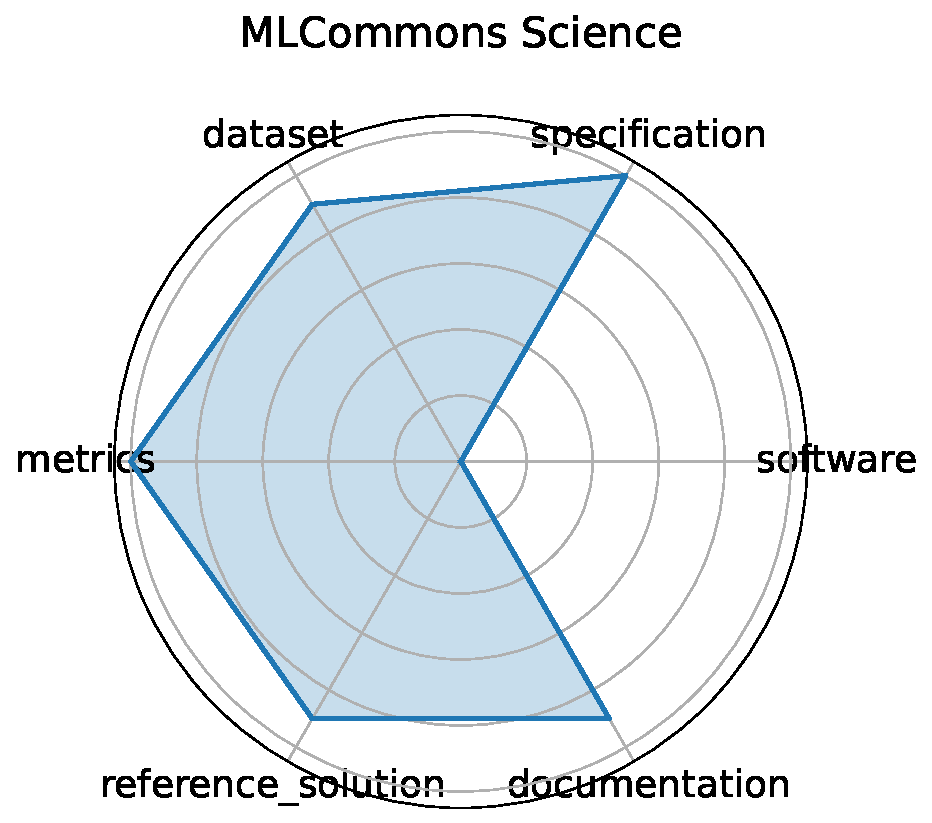
\includegraphics[width=0.2\textwidth]{mlcommons_science_radar.pdf}
\end{description}
}}
\clearpage